\section[Online Analysis]{Online Analysis}
\label{sec:online}

\begin{frame}{Online Analysis}
	\begin{itemize}
		\item Created and simulated the IEEE 9 Bus System in PSSE 34.
		\item Added stochastic disturbance to the loads (at Bus 5, 6 and 8) via white noise modeled as
			\begin{equation}
				(P_L)_{i}[k] = (P_L)_{i}[k-1] + N(0, \sigma^2)
			\end{equation}
		for load bus $i$ at discrete sample $k$.
		$\sigma = 0.01$ pu. 	
		\item In order to drive the power grid towards bifurcation, steadily increased the three loads at different rates, between 20\% to 30\% per minute.
		\item Ran a time analysis simulation until critical bifurcation attained. 
		\item Extracted the bus voltages. 
	\end{itemize}

\end{frame}

\begin{frame}{Online Analysis}
	Passed the voltage signals through a Low Pass Filter in order to capture the slow changing trends not an effect of CSD. 
	Eg. Change in bus voltages due to the gradual increasing of loads.
	Gaussian Kernel Smoothing Filter was used for the same.
	\begin{equation}
	\label{eq:gks}
		h(n, \sigma_f) = \frac{1}{\sqrt{2 \pi} \sigma_f} \exp^\frac{-n^2}{2 \sigma_f^2}
	\end{equation}
	where $\sigma_f$ can be varied between $5$ to $10$ .
	\\ The detrended signal is obtained by subtracting the filtered signal from the original signal.	
	\begin{equation}
	\label{eq:detrending}
		d[x] = x[k] - GKS(x[k])
	\end{equation} 
\end{frame}

\begin{frame}{Online Analysis: Applying AR1 and Variance}
	
	Windows length of $W = 15$ seconds was used for computing autocorrelations and variances.
	The windows were moved by $W_{moving} = 1.5$ seconds after every computation.
	
	For every window, Autoregressive Model of Order 1 was fitted onto the detrended voltages using least squares of error approach.
	\begin{equation}
	\label{eq:autocorrDef}
	d[k] = a_1 d[k-1] + e[k]
	\end{equation} 
	
	Variances were also computed for every window.
	\begin{equation}
	\label{eq:varDef}
	\sigma^2 = \frac{1}{n_k} \sum_{k=1}^{n_k} d[k]^2
	\end{equation} 
\end{frame}

\begin{frame}{Autocorrelations}
	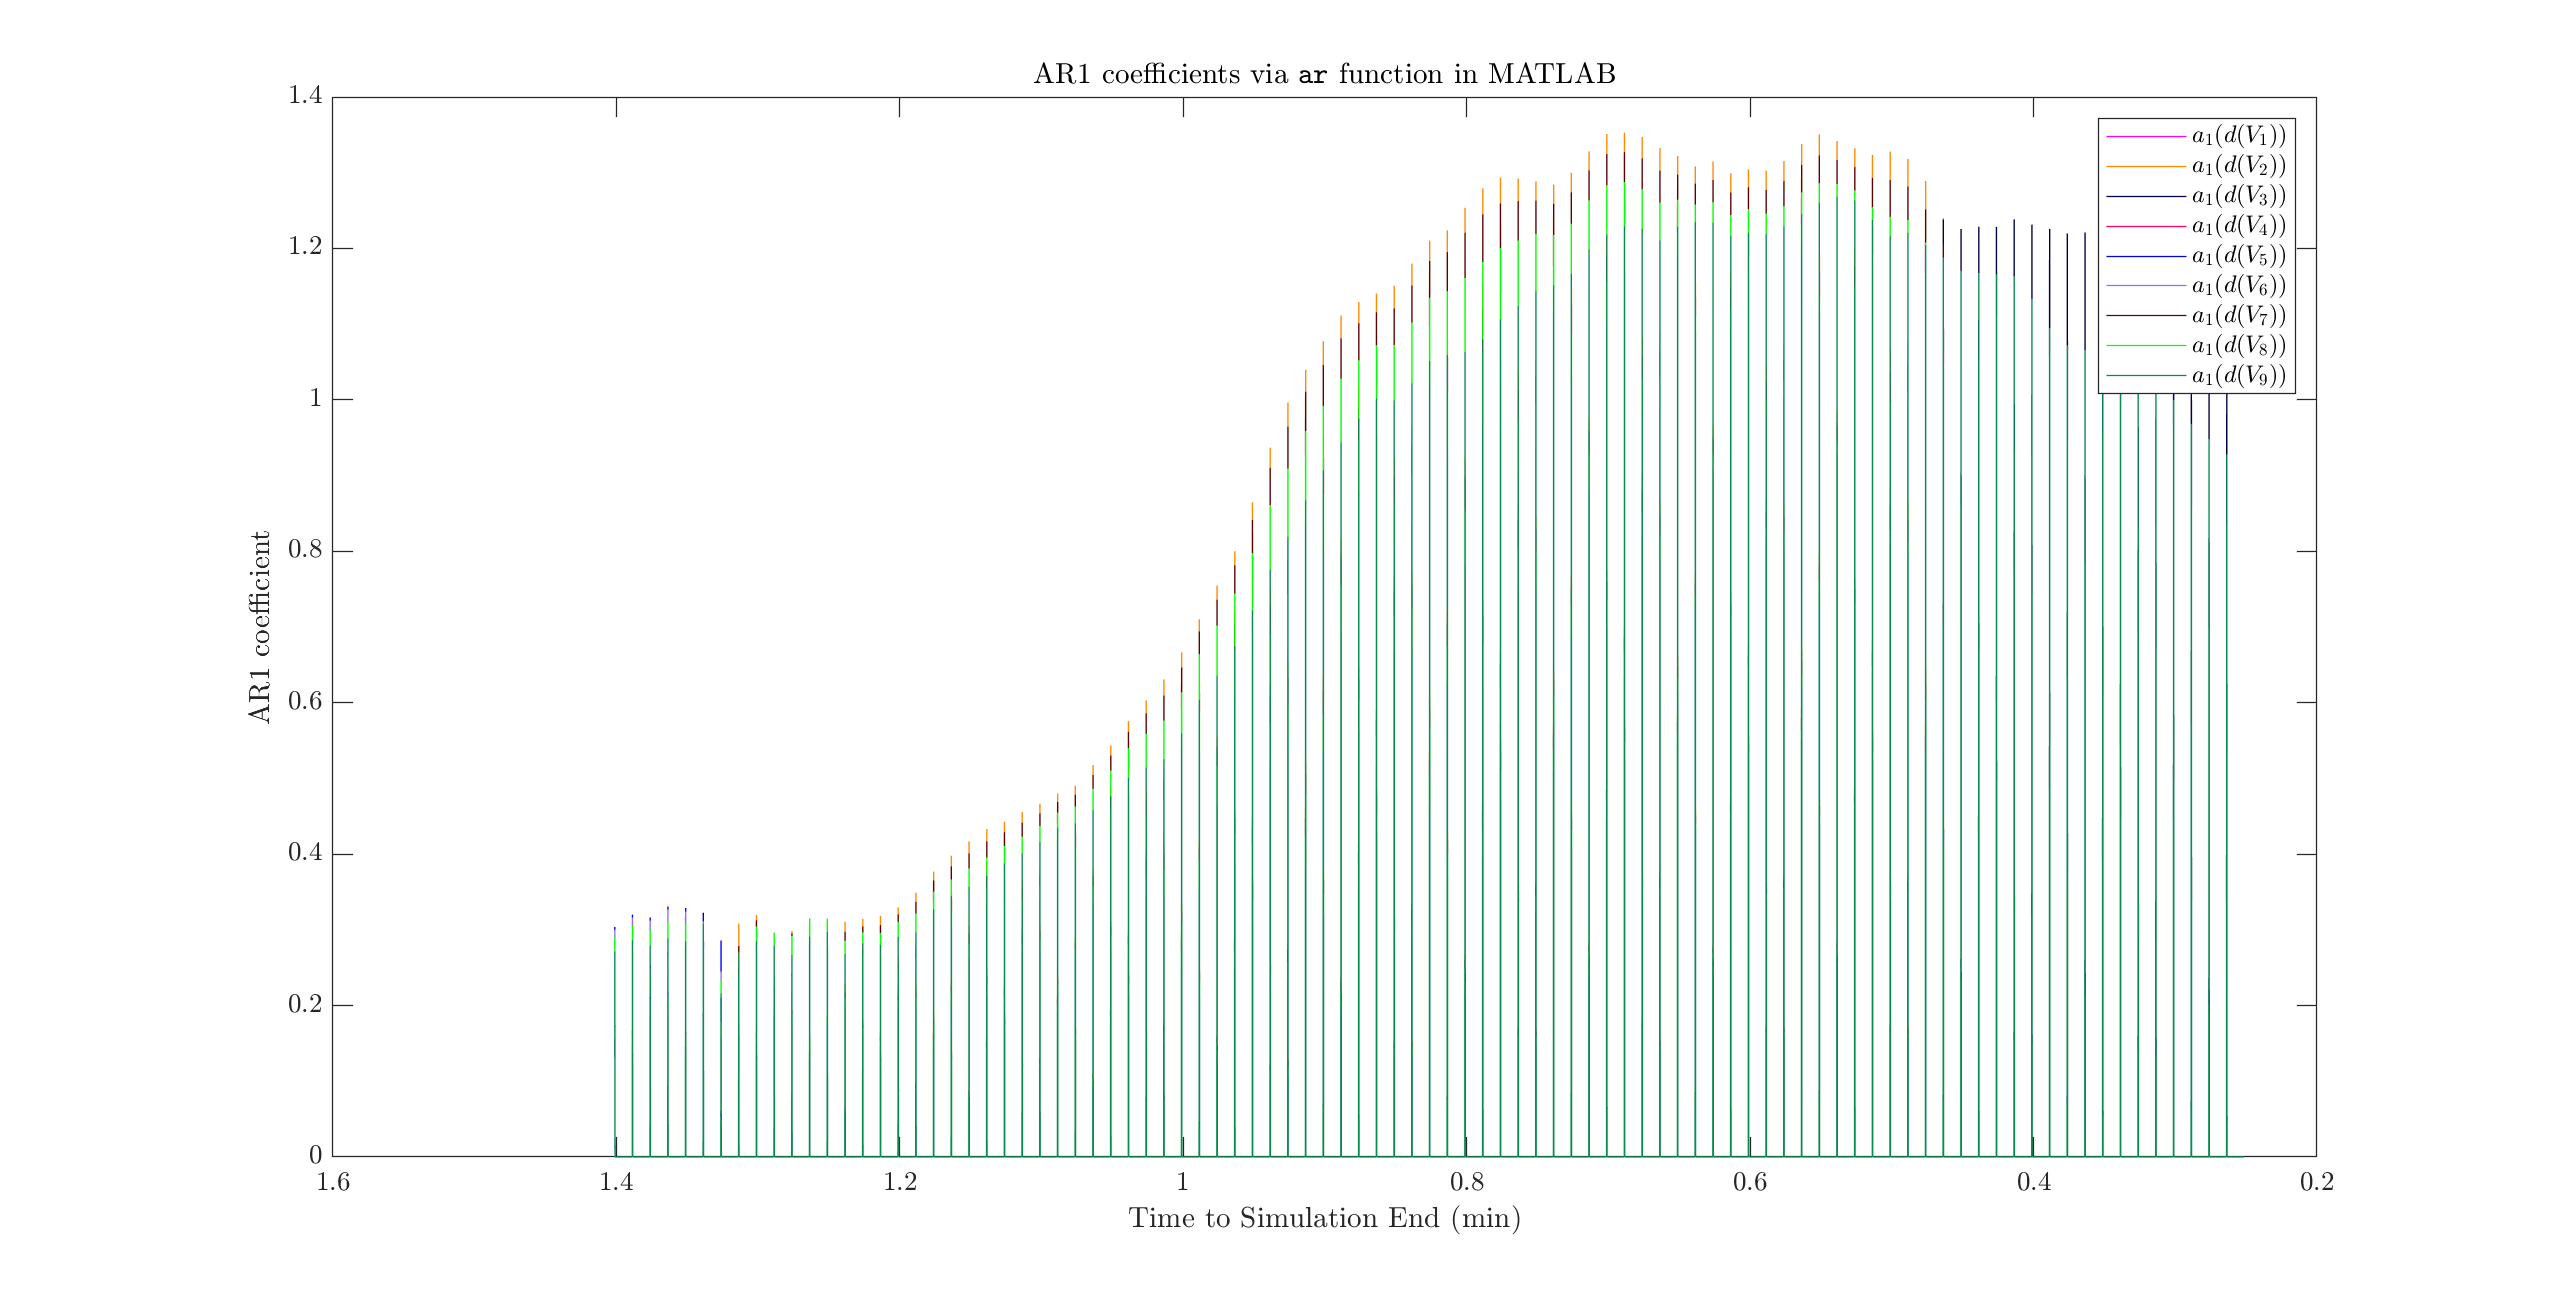
\includegraphics[scale=0.18]{../figures/im01.png}
\end{frame}

\begin{frame}{Variances}
	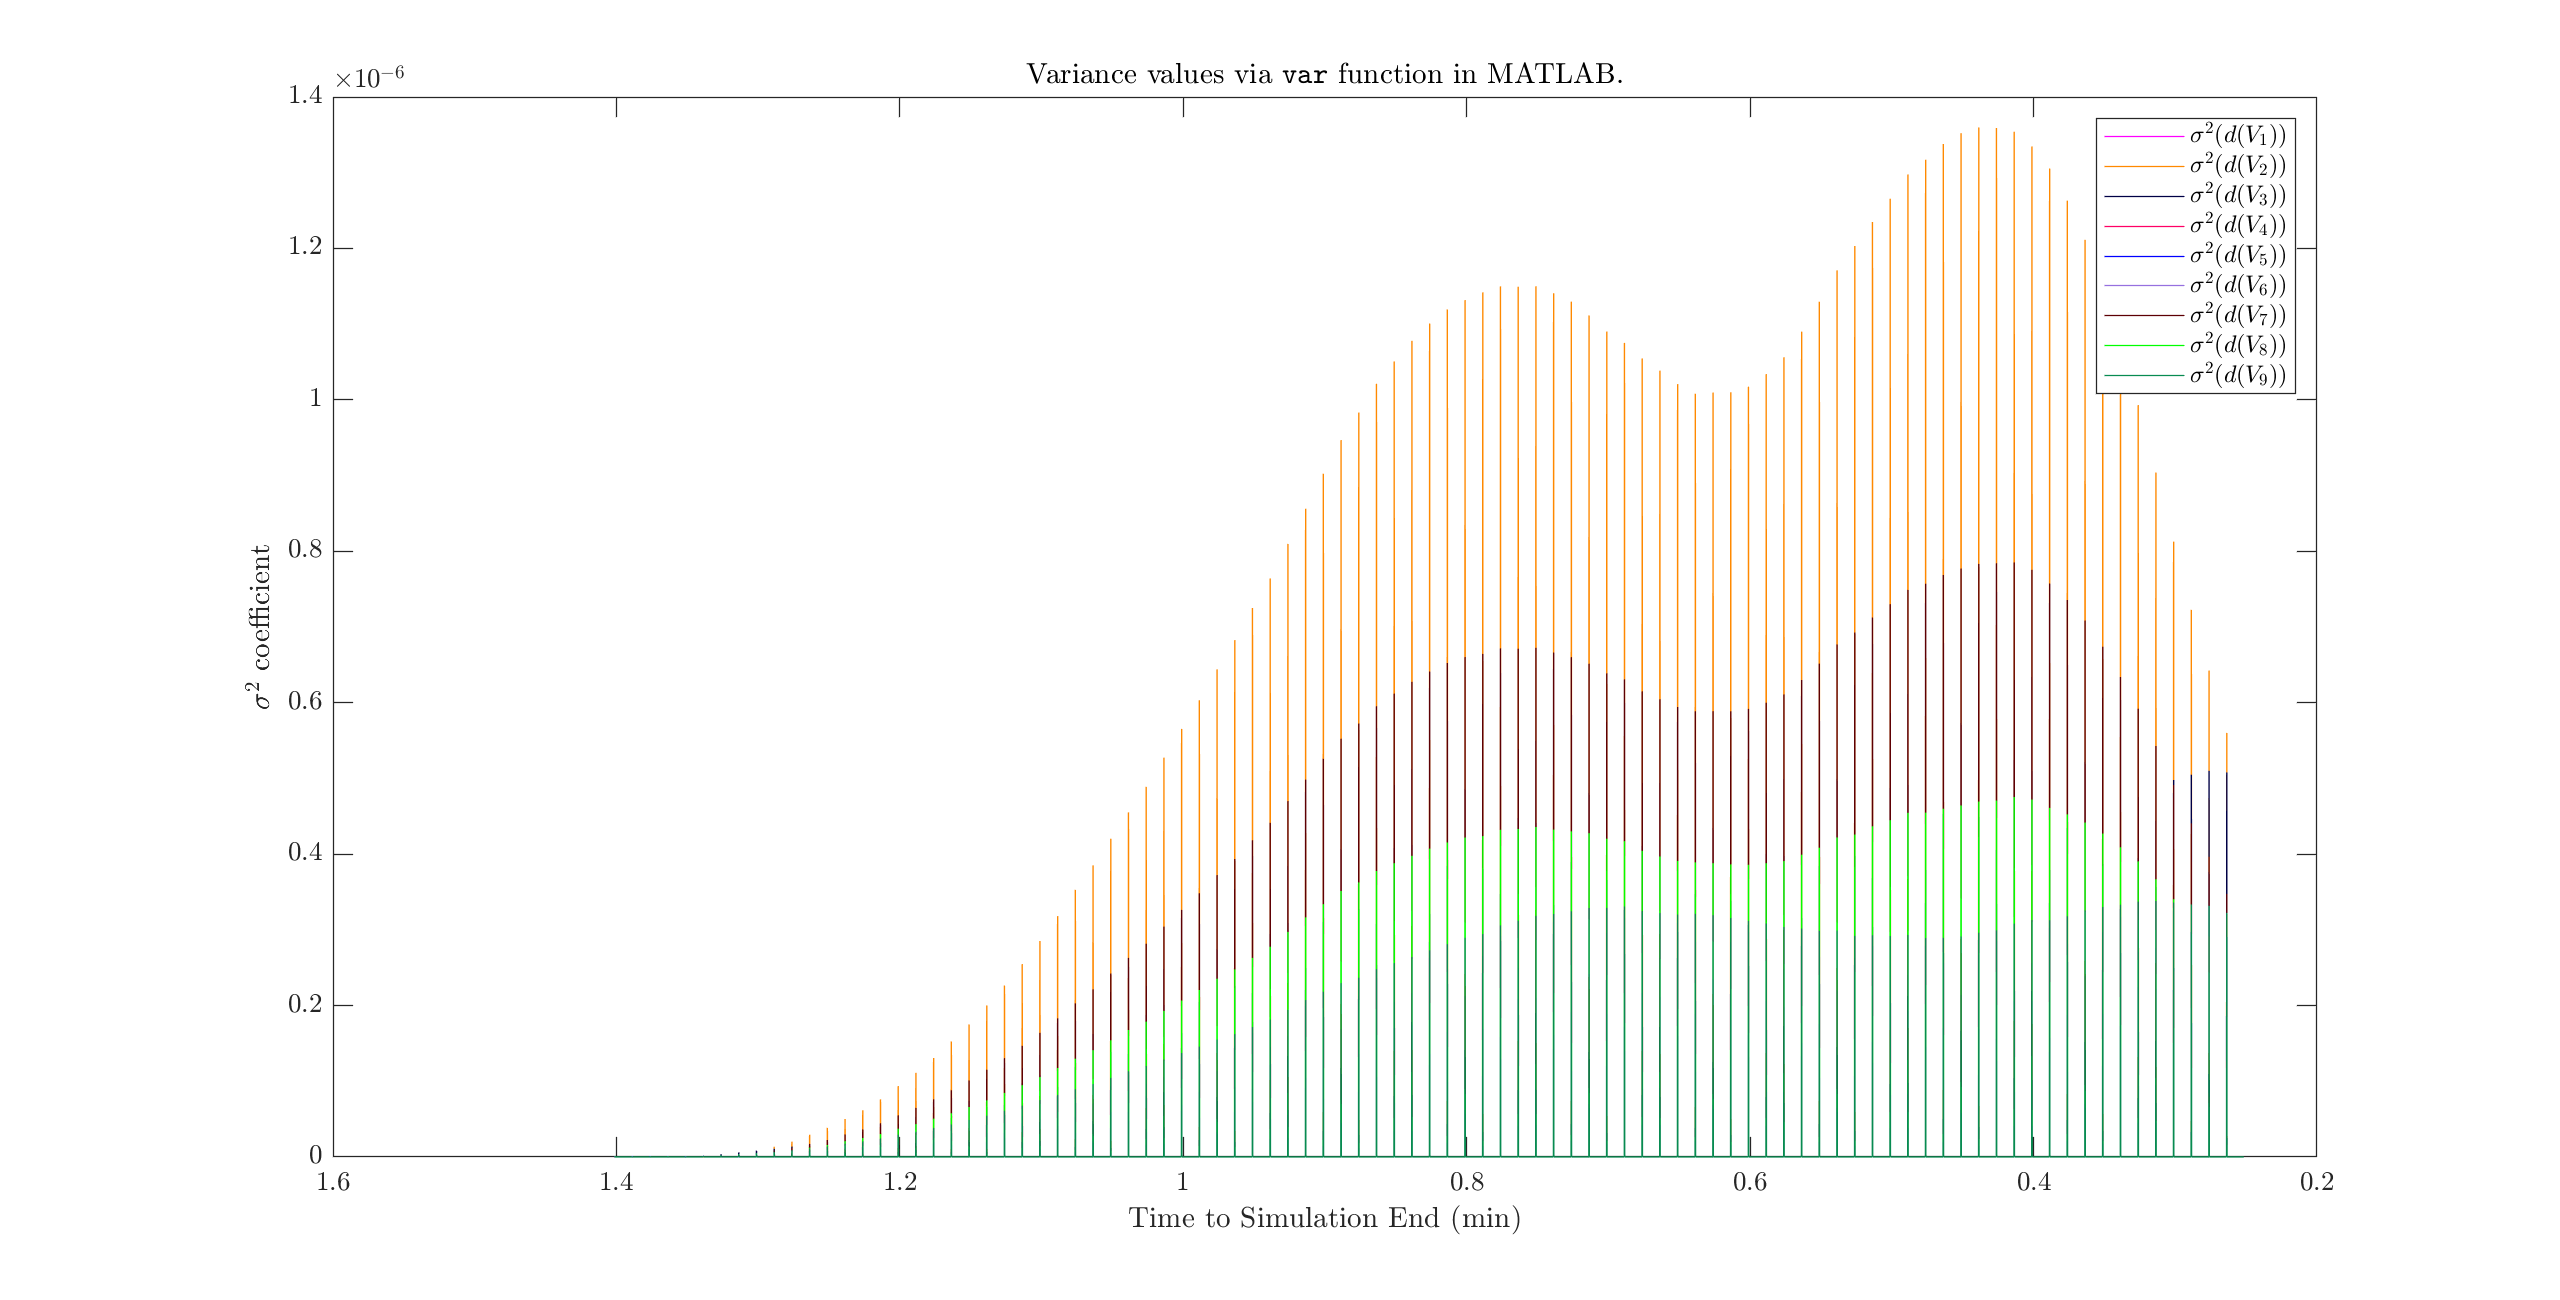
\includegraphics[scale=0.18]{../figures/im02.png}
\end{frame}